% \textbf{Title: Bode Diagram 1}

Consider this Bode diagram.

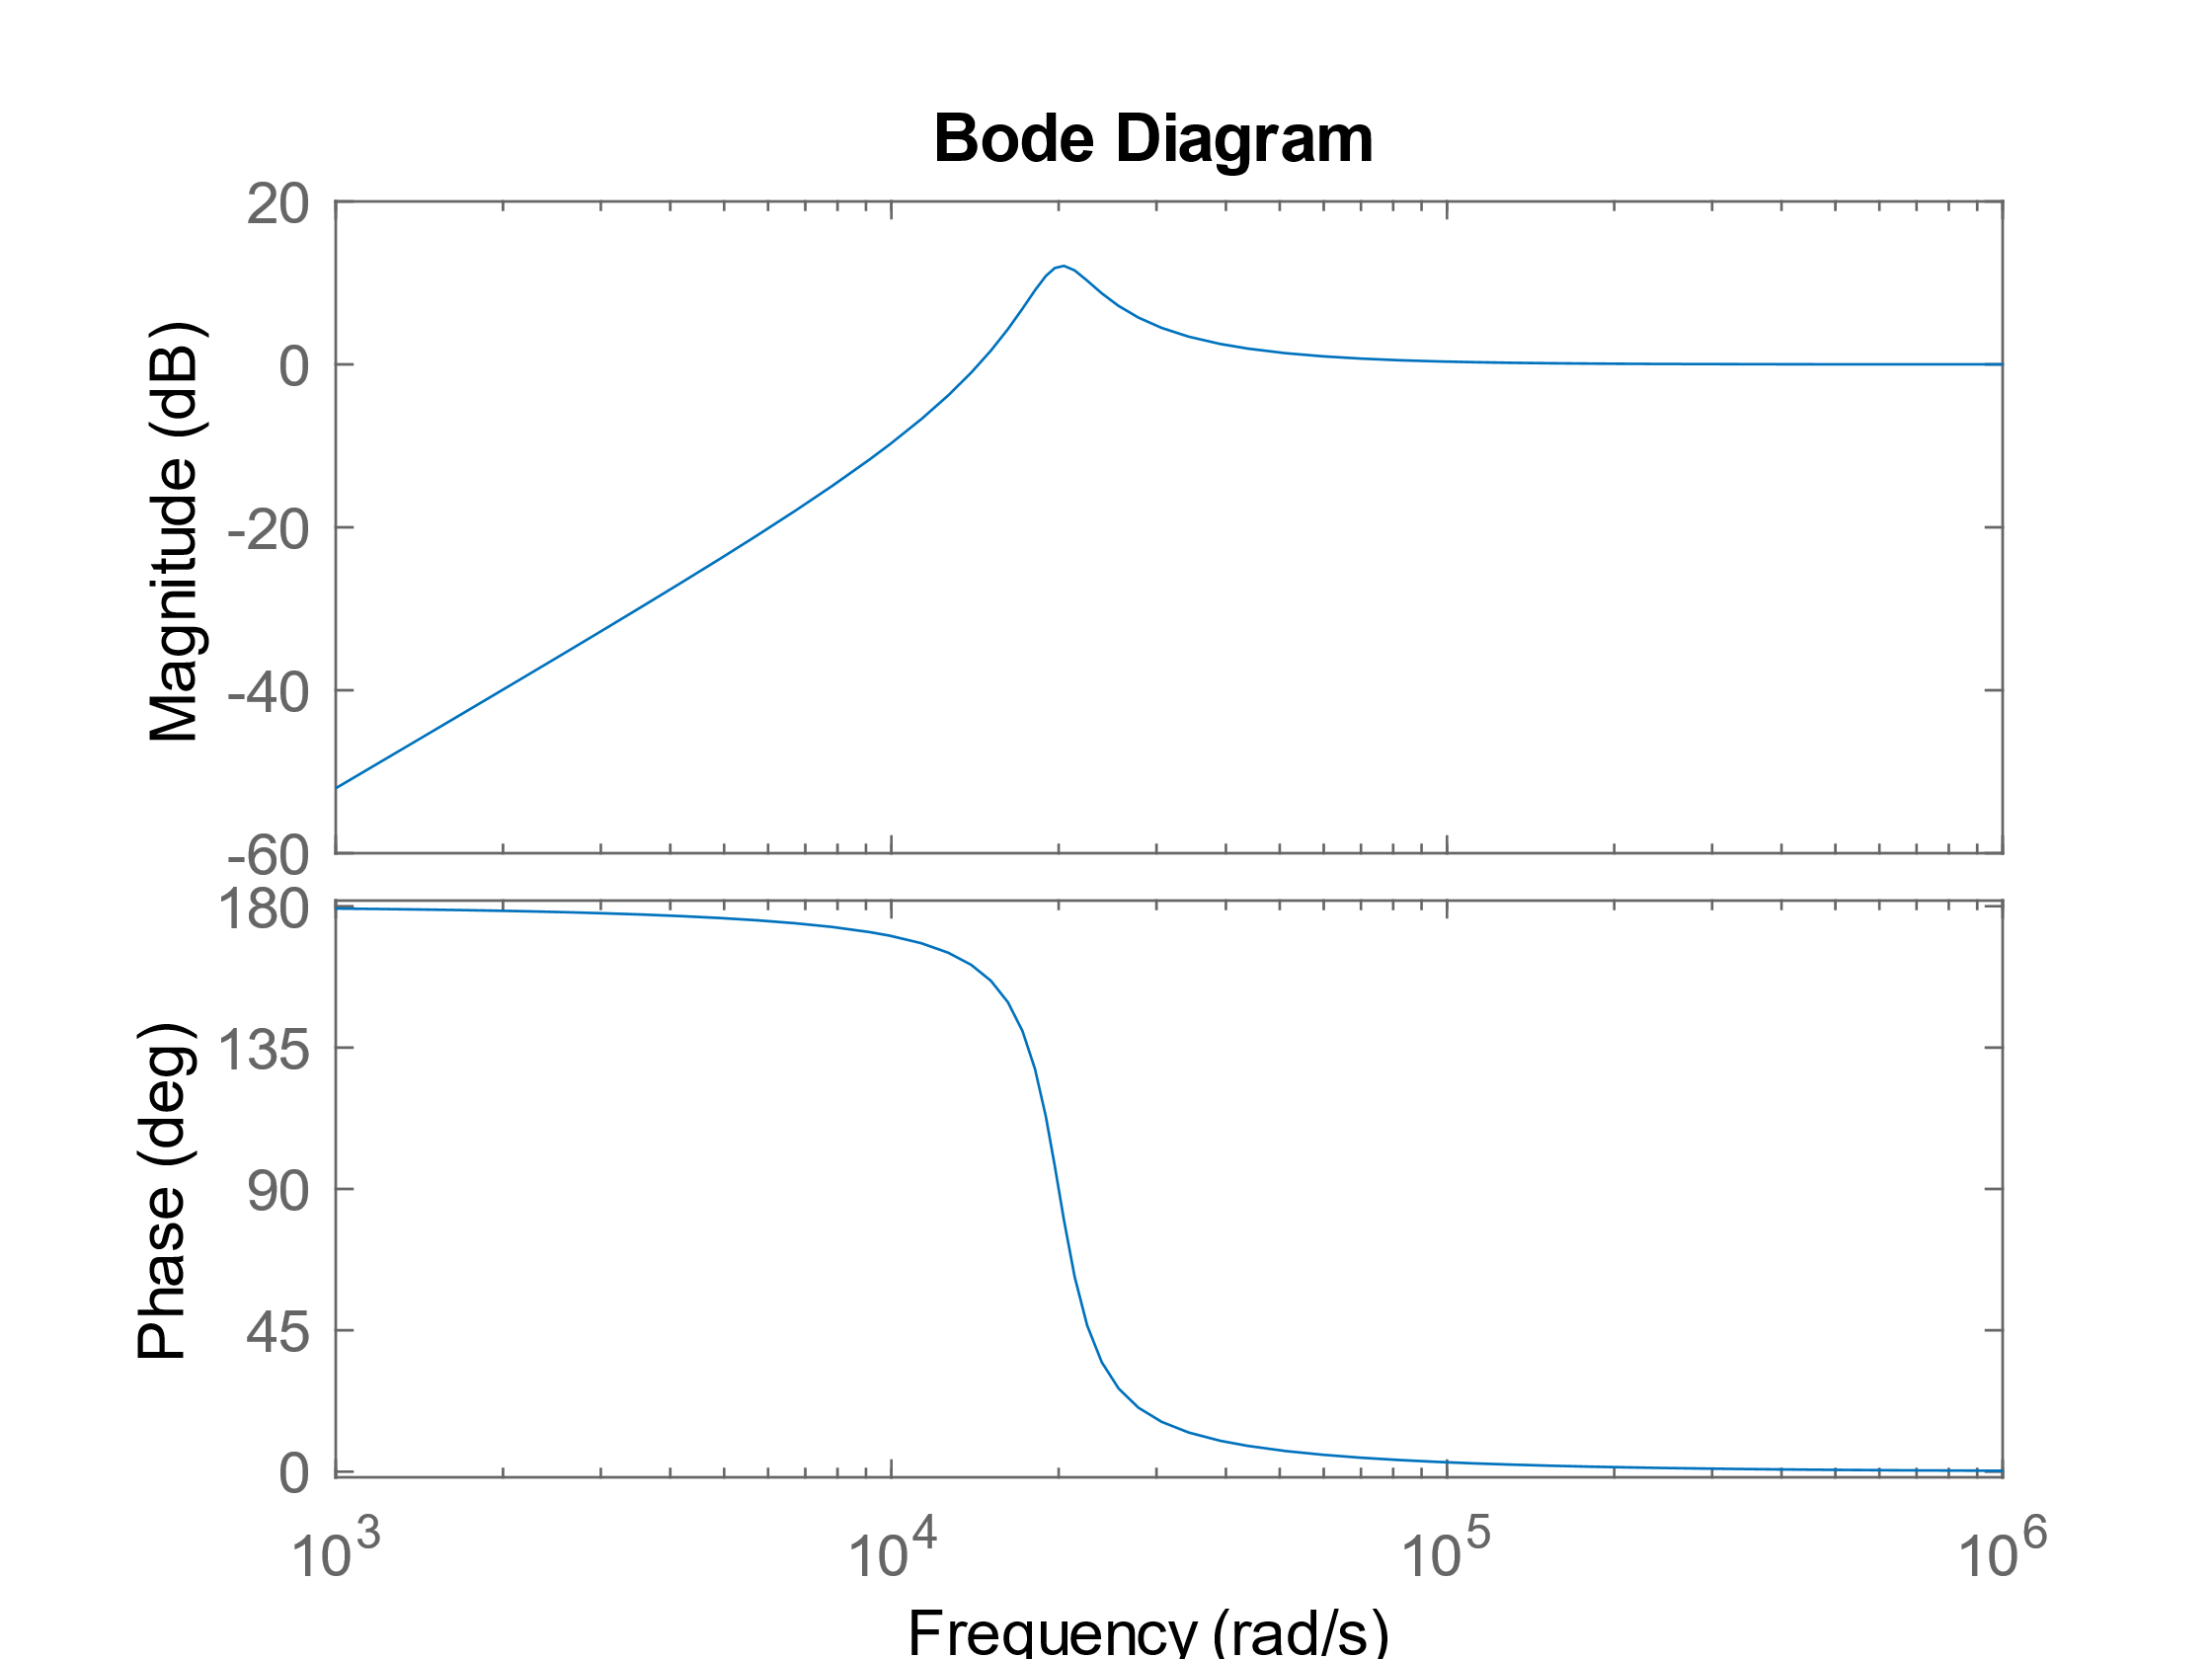
\includegraphics[width=4.64719in,height=3.48617in]{../../Images/BodeDiagramQ1.png}

What can we say about the output signals for input signals of frequencies \(2,000\ \text{rad/s}\), \(20,000\ \text{rad/s}\) and \(200,000\ \text{rad/s}\), respectively?\\

a. The first signal is stopped, the second signal is amplified and the third signal is let through unaffected.

b. The first signal is attenuated and changes sign, the second signal is amplified and phase shifted by \(90{^\circ}\) and the third signal is let through unaffected.

*c. The first signal is attenuated and phase shifted by almost \(180{^\circ}\), the second signal is amplified and phase shifted by \(90{^\circ}\) and the third signal is let through with a slight amplification and phase shift.

d. The first signal is attenuated and phase shifted by almost \(180{^\circ}\), the second signal is amplified and phase shifted by \(90{^\circ}\) and the third signal is let through with a slight attenuation.

e. I do not know.\\
